 \documentclass{IEEEtran}

\usepackage{graphicx}
\usepackage{refstyle}
    \def\RSfigtxt{Fig.\,}%
    \def\RSfigstxt{Figs~}%
    \def\RSFigtxt{Fig.\,}%
    \def\RSFigstxt{Figs~}%

\begin{document}

\title{Generating Realistic Looking Snow Drifts}
\author{William Horn\\University of Alaska Fairbanks\\wbhorn@alaska.edu}
\date{\today}
\maketitle

\section{Introduction}

Last semester in graphics I focused on making a realistic fragment shader for
generating a dynamic snow texture \figref{original} with perlin noise \cite{wiki:perlin}. To
improve the quality of the shader both the efficiency of the shader and the
fidelity will be taken into account.  The initial implementation was just being
rendered on a completely flat plan. It also was very inefficient, because the
normals were calculated every frame, along with another perlin generated texture
to simulate the roughness in the snow.

\section{Previous Research}

To initially make realistic snow I used a glsl implementation of perlin
\cite{noiseglsl} to generate random normal vectors to represent the orientation
of the snowflake. Due to the fact that which face of the snowflake was being
used to reflect the light, normals were only calculated in the positive
hemisphere. To accomplish this took 2 perlin random numbers to generate a normal
at a point on the plane. The normals were then used to calculate the specular
highlight in the blinn phong illumination model \cite{blinn1977models}.  This
was used to create a sparkle when the user moved around the scene.

To get around the fact that the diffuse component was being ignored a texture
was used in its place. Perlin noise was again used to generate a 1/fnoise
pattern to simulate the roughness in the snow \figref{fnoise}.  This
created a nice rough texture that was used to simulate both the large, and the
small deformities in the snow.

To generate a realistic snow texture, there are three components that I thought
to try an simulate.  First, and at the most micro scale, is the sparkling of the
snow. Whenever the view of the viewer changes, the snow glints creating a sea of
sparkles at varying degree. There were two main challenge I found when trying to
find an implementation for this, the granularity of the sparkle and creating a
natural change in the sparkle with movement.  When the view moves each snowflake
fades in and out of sparkle smoothly.  This is why I initially choose perlin
noise to generate the random normals, looking back however I believe that this
effect would have been taken care of by the blinn phong model if the normals
were truly random as long as the normals were at a large enough resolution to
show up as sparkles. The next challenge was to get the sparkles to look like
snowflakes.  The perlin technique can accomplish this but it doesn't allow for
fine grained control over the size of the sparkle.

Lastly the drifting of the snow must be taken into account. There was no simple
way to implement this, due to the fact that to calculate and render such complex
volumes was out of the immediate scope of my expertise. So to imitate this I
used the 1/fnoise texture \figref{fnoise}. The larger color variations
are used for this. The next component is the variation on the surfaces of the
snow itself.


\section{Background Problem}

Improvements in efficiency will come from the implementation of some of the to
make the sand dunes sparkle \cite{journey}. While this is a different medium,
the same concepts apply because the desired effect is so similar and the
techniques they used to implement it are still very applicable.

To improve the method for rendering the glints in the snow techniques for
rendering multi scale surfaces are used \cite{multiscale}. Although adding some
volume to the snow drifts.


\section{Proposed Solution}

Talk about what you are going to do/did

% myresearch is the file myresearch.bib where you copy/paste all your BiBTeX references
\bibliographystyle{alpha}
\bibliography{project0}

\begin{figure*}
  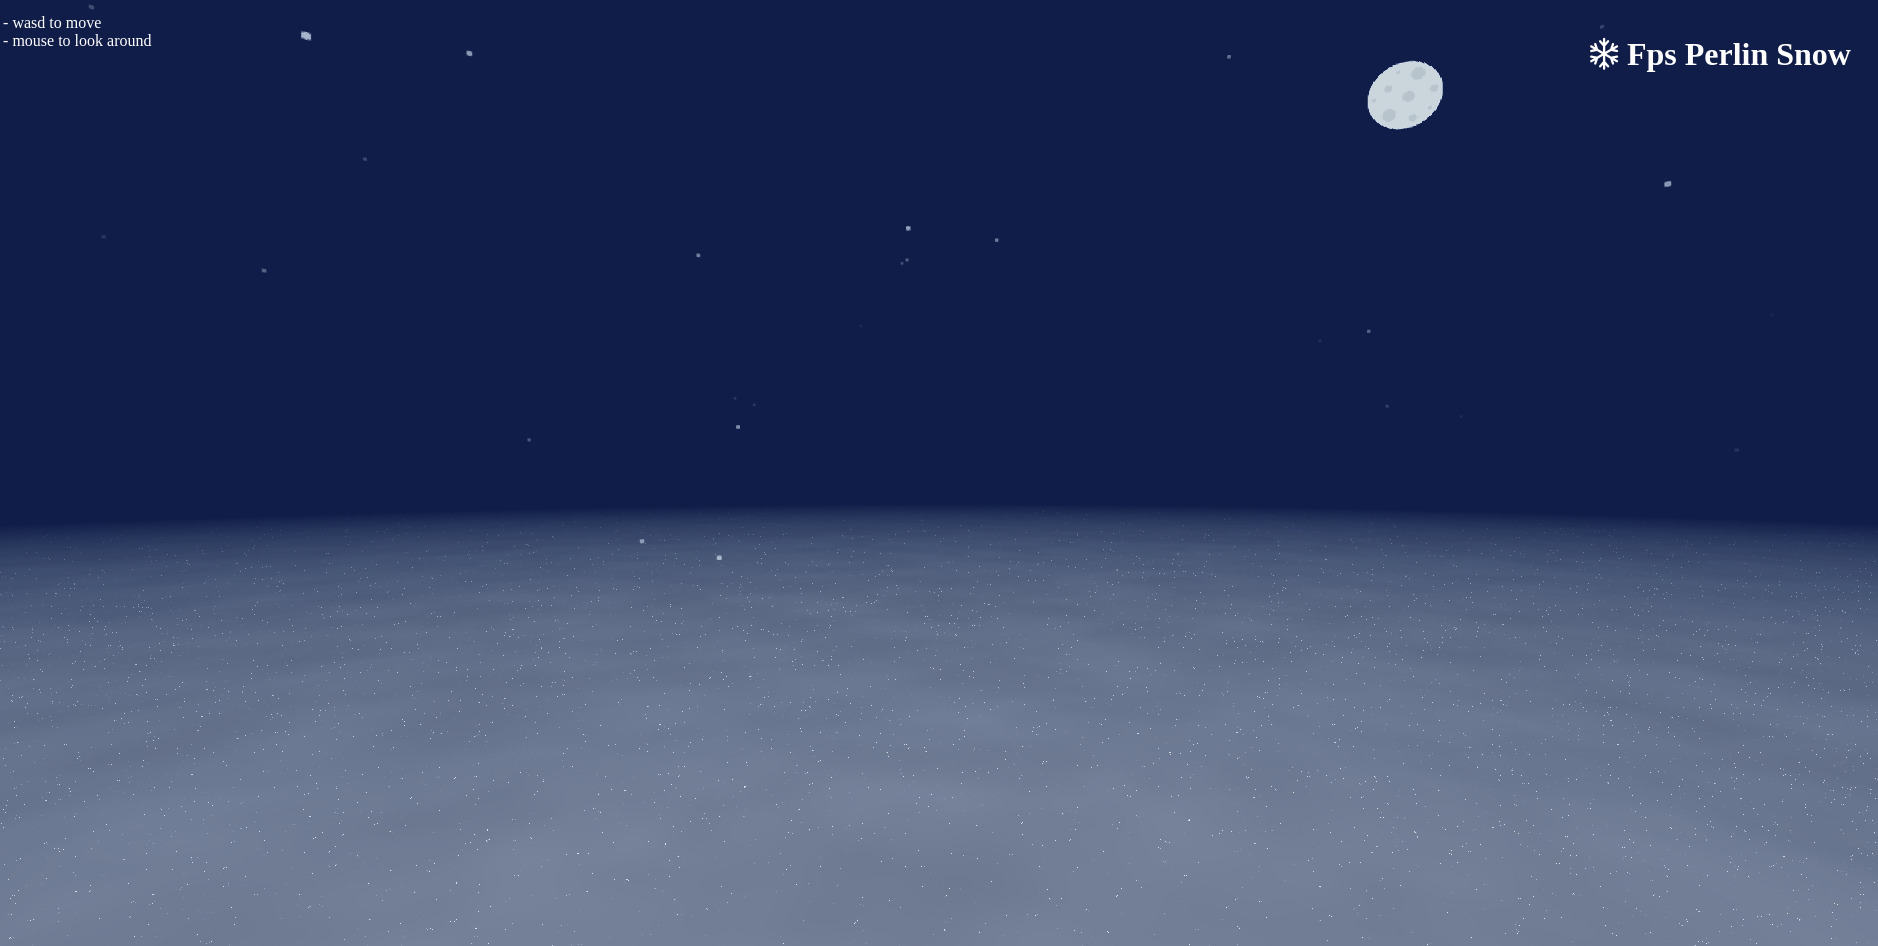
\includegraphics[width=\linewidth]{original.jpg}
  \caption{Original implementation for dynamic snow texture}
  \label{fig:original}
\end{figure*}

\begin{figure*}
  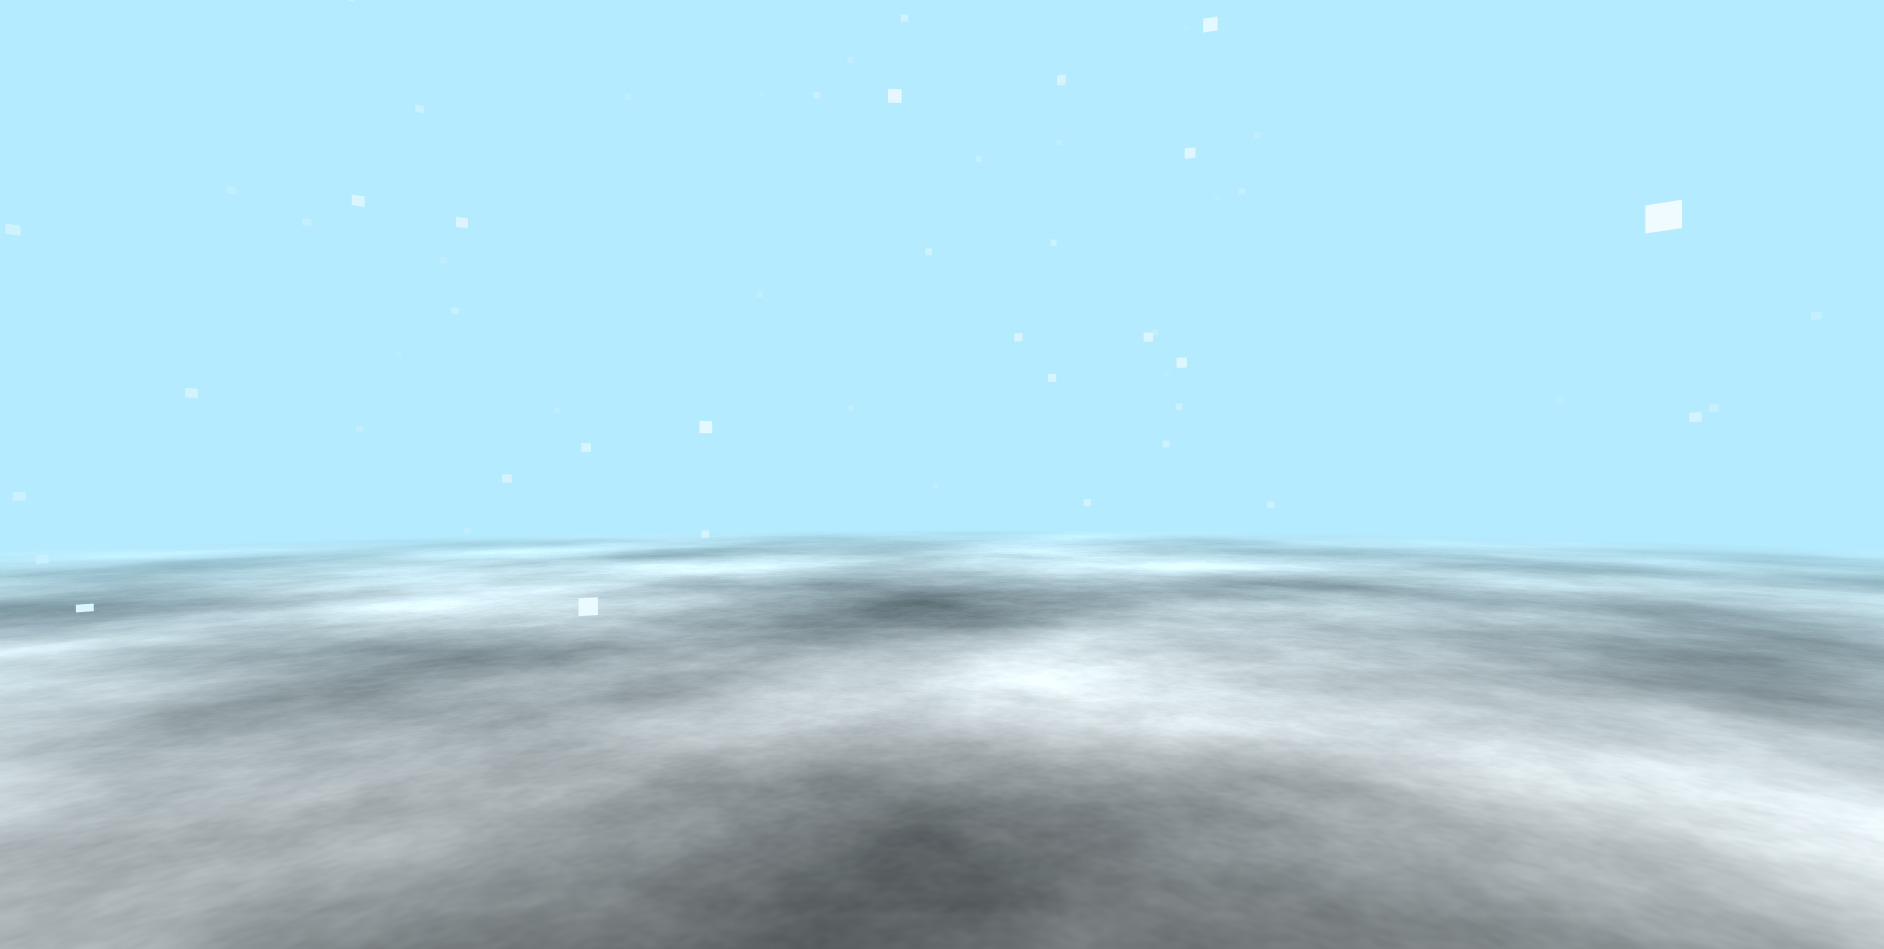
\includegraphics[width=\linewidth]{fnoise.jpg}
  \caption{Plain 1/fnoise pattern from original implementation.}
  \label{fig:fnoise}
\end{figure*}


\end{document}
